\section{System Overview} \label{sec:overview}
\begin{figure}
    \centering
    \framebox[\columnwidth][c]{
        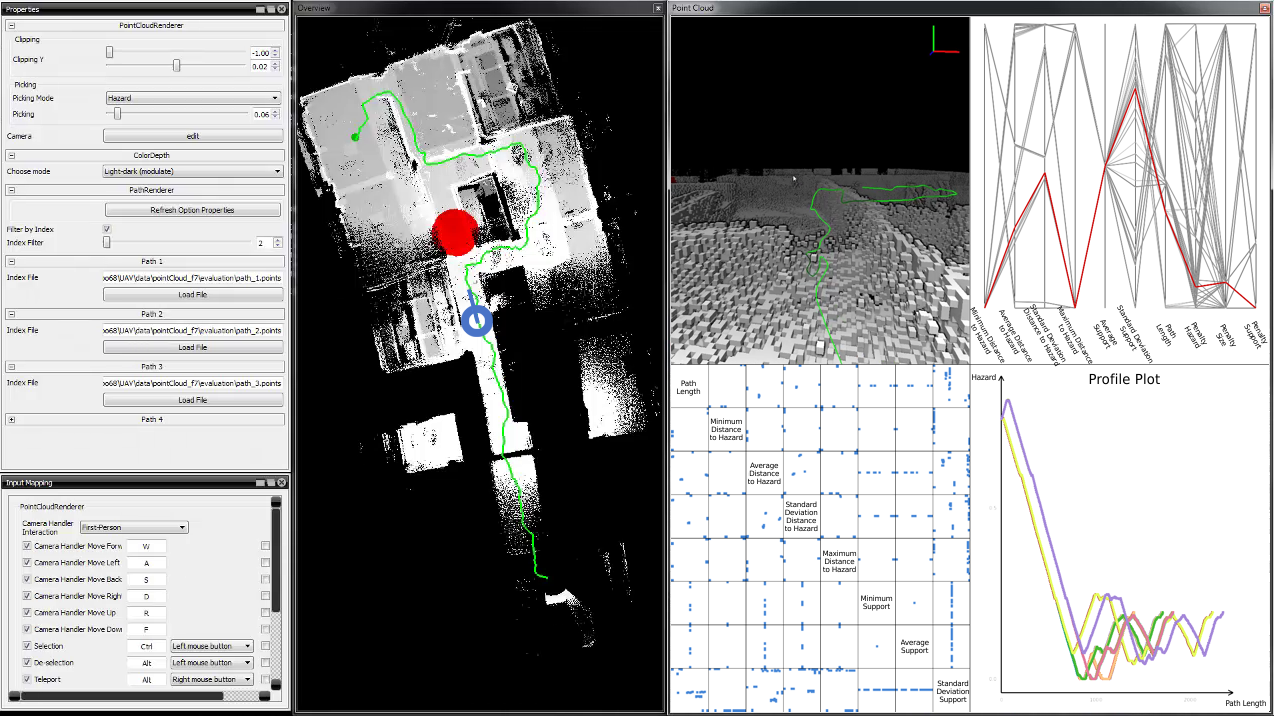
\includegraphics[width=\columnwidth]{figures/fig-overview-system2.png}
    }
    \caption{A screenshot showing our system using usage. The overview map is shown in the middle with the current camera position marked. The right view allows or detailed inspection and navigation. Each subview can be maximized.}
    \label{sec:overview:system}
\end{figure}

In order to fulfil requirement {\bfseries R1}, our system presents the acquired point cloud as an interactive 3D rendering, which preserves occlusion and allows the \IC\ to form a mental model of the structure. In this rendering environment, the \IC\ can seamlessly annotate newly discovered entrances, hazards, and POIs, thus fulfilling requirement {\bfseries R2}. To address requirements {\bfseries R3} and {\bfseries R4}, we provide renderings of the different paths integrated into the 3D rendering as well as separate, in-depth analysis tools.

The following subsections explain the individual parts of the proposed system. The data preprocessing that extracts derived data from the point cloud is described in Section~\ref{sec:overview:precomputation}. The data annotation is illustrated in Section~\ref{sec:overview:classification}. The computation of the ensemble of paths, and the metric used, is described in Section~\ref{sec:overview:path} while Section~\ref{sec:overview:analysis} deals with the support of the analysis of these paths. Section~\ref{sec:overview:rendering} explains the considerations that went into the rendering.

\subsection{Data Preprocessing} \label{sec:overview:precomputation}
\begin{figure*}
    \newlength{\mysize}
    \setlength{\mysize}{0.35\columnwidth}
    \centering
	\subfigure[Hazard field]{
	    \framebox[\mysize][c]{
	        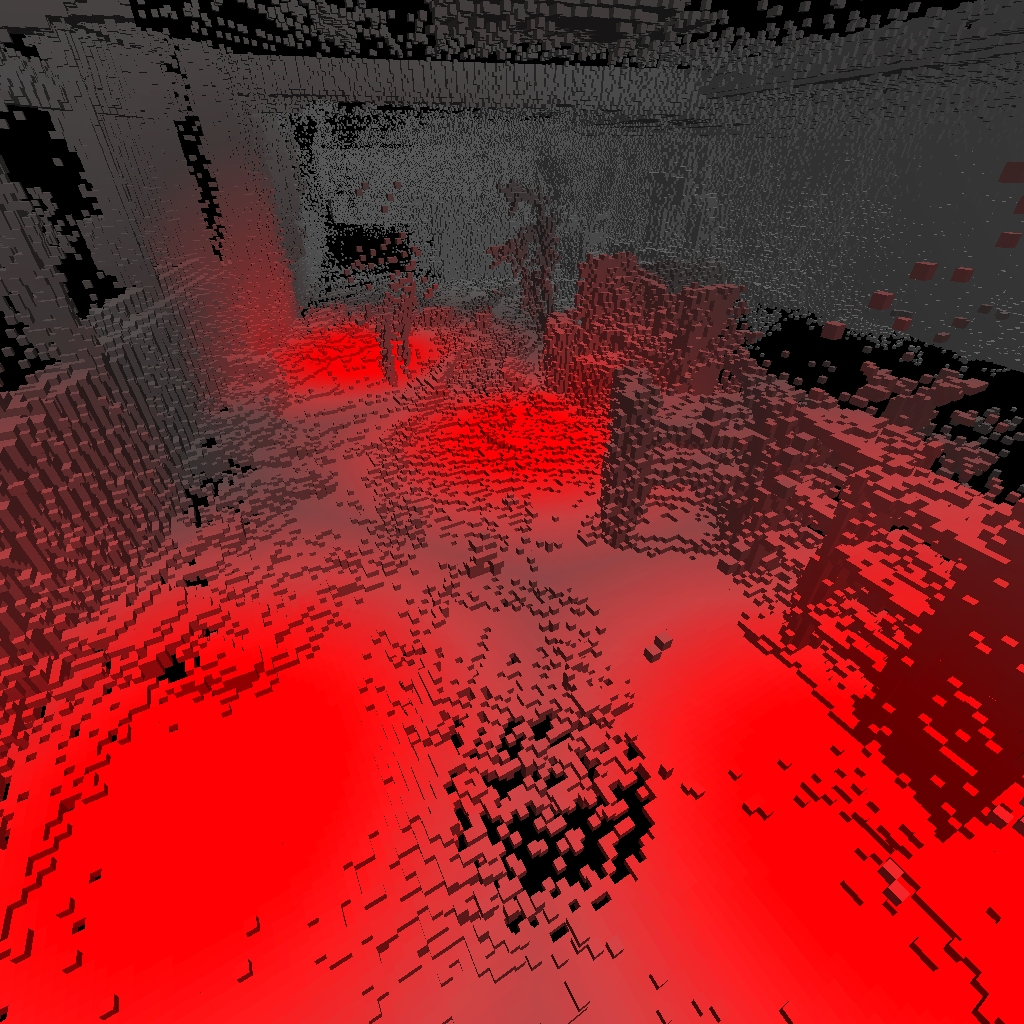
\includegraphics[width=\mysize]{figures/fig-overview-hazardfield.jpg}
	    }
	    \label{fig:overview:precomputation:hazardfield}
	}
	\subfigure[Support field]{
	    \framebox[\mysize][c]{
	        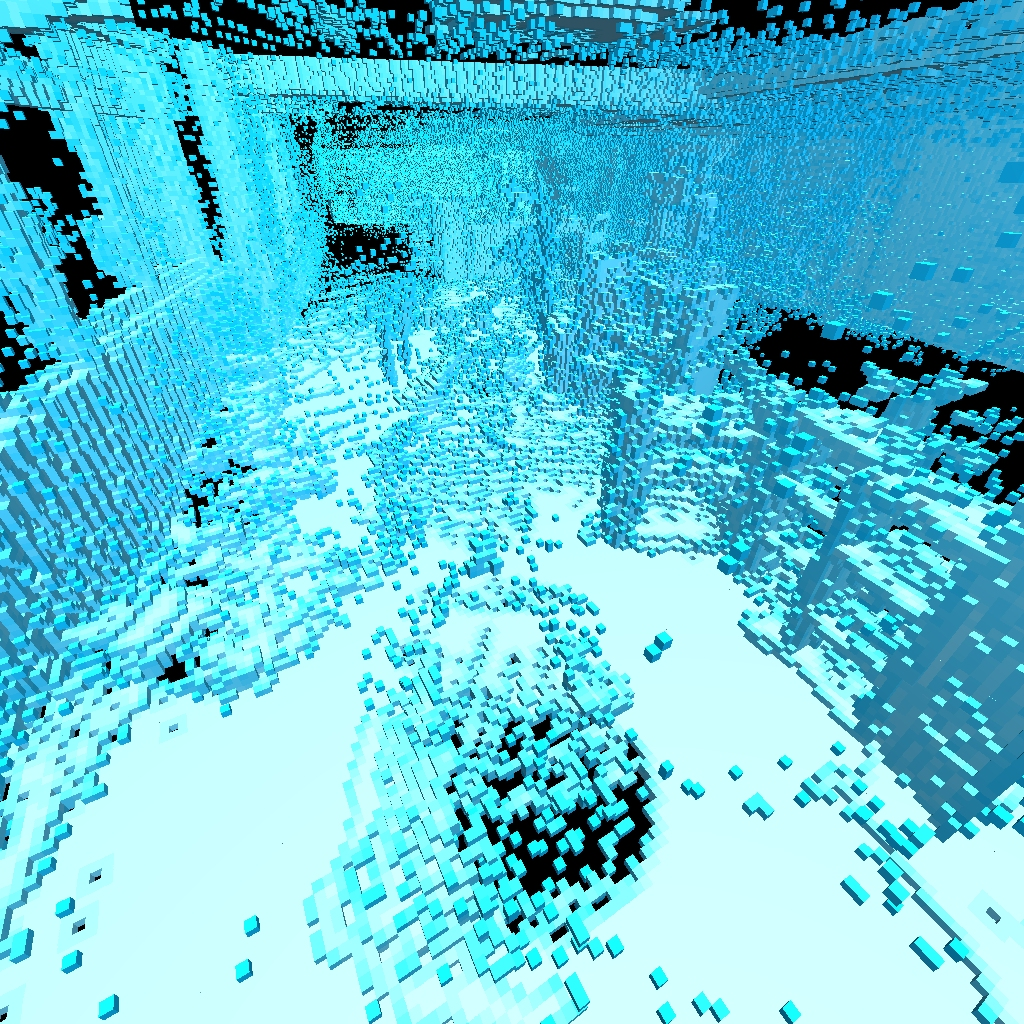
\includegraphics[width=\mysize]{figures/fig-overview-supportfield.jpg}
	    }
	    \label{fig:overview:precomputation:supportfield}
	}
	\subfigure[Occupancy field]{
	    \framebox[\mysize][c]{
	        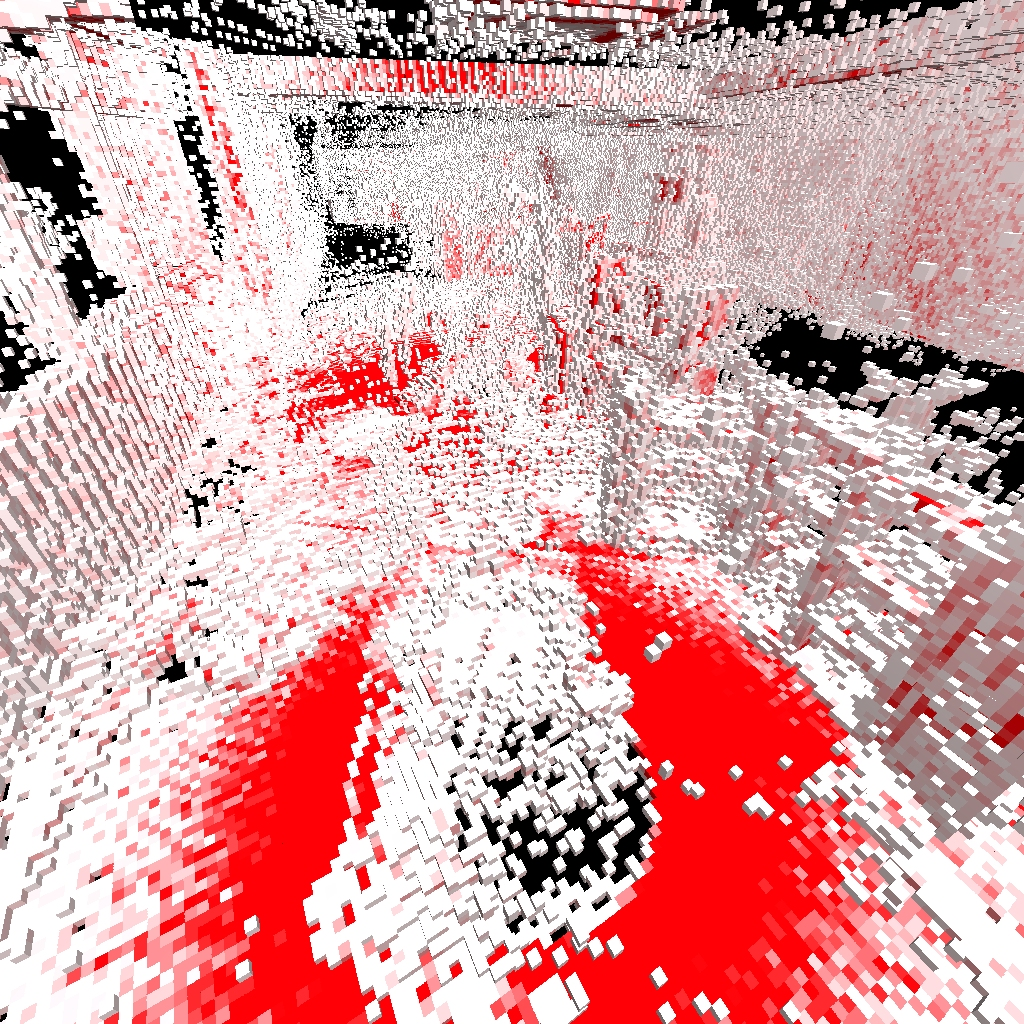
\includegraphics[width=\mysize]{figures/fig-overview-occupancyfield.jpg}
	    }
	    \label{fig:overview:precomputation:occupancyfield}
	}
	\subfigure[Size field]{
	    \framebox[\mysize][c]{
	        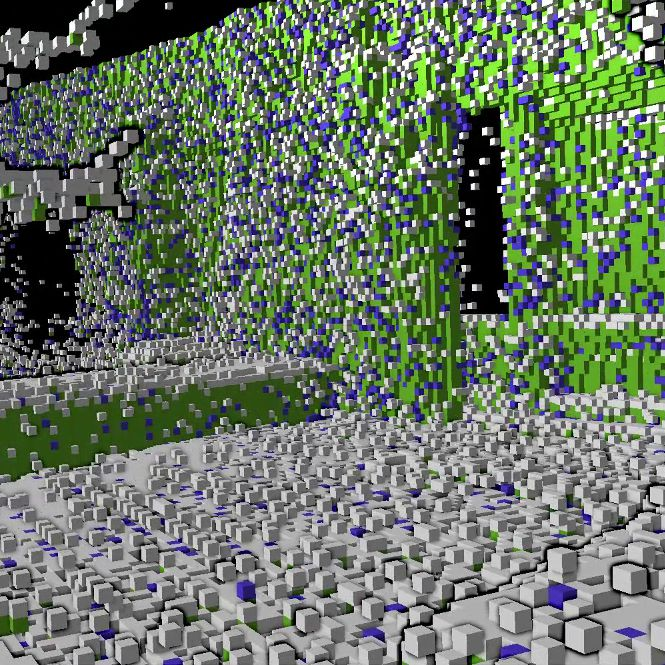
\includegraphics[width=\mysize]{figures/fig-overview-sizefield.jpg}
	    }
	    \label{fig:overview:precomputation:sizefield}
	}
	\caption{Three of the derived attributes are mapped to the individual voxels and are shown: (a) closest distance to hazard, (b) level of support, (c) occupancy, or data density, and (d) the availability of space above each voxel.}
    \label{fig:overview:precomputation}
\end{figure*}

\noindent {\bfseries Scan conversion.} The data retrieved from the unmanned robots is an unstructured 3D point cloud of the interior of the collapsed building. The resolution of the scan is highly dependent on the allotted scanning time as well as the employed scanner. One issue with point rendering is missing occlusion information. To avoid this problem, we perform a binning of the point cloud to obtain an axis-aligned voxel data structure. The necessary voxel size is highly dependent on the scan resolution of the robot, as it is a trade-off between resolving smaller details versus increasingly noisy data. In our test case, voxel sizes of $5$cm were sufficient with regard to this trade-off. The resulting grid-based data structure contains one voxel for all bins with the occupancy exceeding a certain threshold. In our approach, we discard every voxel that only depends on a single measurement point, since this is likely due to measurement noise. From this point on we refer to a \emph{point} in the original point cloud and to a \emph{voxel} in the binned point cloud.

\noindent {\bfseries Parameter derivation.} Derived attributes are computed for the voxel data, which are subsequently used to determine a set of viable rescue paths and to support filtering of these paths. We compute a \emph{distance field} (Figure~\ref{fig:overview:precomputation:hazardfield}) that denotes the distance to the closest hazard points, weighted by severity, for each voxel. Let $\mathbf{i}$ be the current voxel, $H$ the set of hazard points, and $H^{\mathbf{i}}_s$ the normalized severity for $\mathbf{i}$, then the hazard field is given by: $h(\mathbf{i}) = \min_\mathbf{j}(\mathrm{L}_2(\mathbf{i}, H^\mathbf{j}) \cdot H^\mathbf{j}_s)$. The \emph{support field} (Figure~\ref{fig:overview:precomputation:supportfield}) shows the available supporting area for each voxel. This value determines if there is enough floor available for a responder to walk unhindered. The voxel neighborhood in the plane perpendicular to the gravity axis is considered as that plane coincides with horizontal surfaces. The \emph{occupancy field} (Figure~\ref{fig:overview:precomputation:occupancyfield}) denotes the number of  points each voxel is based on. A higher occupancy means that the voxel contains more points in the original point cloud data and thus provides a higher certainty. The occupancy can be increased by longer scan rates and better scanning technology. The \emph{size field} (Figure~\ref{fig:overview:precomputation:sizefield}) shows for each voxel if a rescuer can fit into the space above without squeezing. We calculate two size values, one with the rescuer standing up and a second while crouching.

To compute viable paths, we need orientation information to be able to exclude paths that would be to steep for a rescuer. We utilize data normals in order to indicate the orientation of structures of interest. We investigated two sensible measures for determining the normal direction at each voxel. In the first method we compute the least-squares fitted plane based on all the points that a voxel covers. The normal of the resulting plane is used as the normal for the voxel. The second method performs a least-squares fit of the neighborhood of the voxel to determine the principal direction of the plane. In our tests we found that the first method results in greater stability provided higher occupancy.

\subsection{Data Annotation} \label{sec:overview:classification}
With respect to requirement {\bfseries R2} it is essential for the \IC\ to be able to classify and annotate the data. Each voxel can belong to one of five classes. \emph{Unclassified} is the default type for all voxels. \emph{Start} voxels are entry points, which the \IC\ has declared as accessible. This means that each path can start from any of these set of points. \emph{POI} voxels are denoted, either by the robots or by the \IC, to be destination points for a path. \emph{Hazard} voxels have been declared as dangerous due to, for example, an ongoing fire or gas leak. Each hazard area has a severity that denotes how important it is to avoid it. \emph{Forbidden} voxels can only be declared by the user and are areas completely out of reach for traversal. These points are used when, for example, a corridor collapses and is not accessible anymore.

The \IC\ can modify the classification for each voxel by interacting with the rendering of the point cloud. He can either modify a single point or perform a radius-based selection of all nearby points close to the selection. 

\subsection{Path Computation} \label{sec:overview:path}
For the path computations we make use of the widely used A* algorithm~\cite{4082128}. It is a best-first search algorithm that uses the L$_2$ distance as a heuristic to estimate the distance to the target. The algorithm works as follows. For the current point $x$ all unvisited neighboring points $y_i$ have the estimated remaining distance calculated. This value is the sum of the cost to reach $x$, the cost to move from $x$ to $y_i$, and the estimated cost to reach the target. These points are inserted into an open list and the point with the lowest cost is chosen as the next valid point; the current point is then removed from the open list and marked as visited. For a comprehensive description of the algorithm we refer the reader to~\cite{AStar}.

The metric determines the cost of moving from one point to its neighbor. Thus, it is possible to compute several optimal paths by changing the metric that is used for the A* algorithm. While it is possible to change the metric during the computation, we did not include this into our system as the resulting complexity in interaction would be prohibitive for the \IC. The metric that is used in our system is composed of several, weighted submetrics that are summed up to yield the metric $m$

\begin{eqnarray*}
m & = & \textrm{distance}(\mathbf{p},\mathbf{q}) + w_h \cdot \textrm{hazard}(\mathbf{q}) + w_s \cdot \textrm{size}(\mathbf{q}) + \\
  & & w_n \cdot \textrm{normal}(\mathbf{q},\varphi) + w_{sup} \cdot \textrm{support}(\mathbf{q},n)
%m = & w_d \cdot distance(p,q) + w_h \cdot hazard(p,q) + \\
%  & w_n \cdot normal(p,q,angle) + w_s \cdot size(p,q,type) + \\
%  & w_o \cdot overhang(p,q) + w_{sup} \cdot support(p,q,area,n)
\end{eqnarray*}

\noindent where $w_{h,n,s,sup}$ are the weights that are varied between different runs, of the path computation. $\mathbf{p}$ is the current point, and $\mathbf{q}$ is the point under consideration.

The function $\textrm{distance}(\mathbf{p},\mathbf{q})$ calculates the L$_2$ distance between points $\mathbf{p}$ and $\mathbf{q}$ with the result in standard units. $\textrm{hazard}(\mathbf{q})$ returns the hazard severity. $\textrm{size}(\mathbf{q})$ is a binary function that determines if there is enough space above the voxel $\mathbf{q}$. The $\textrm{normal}(\mathbf{q},\varphi)$ function computes the surface normal for $\mathbf{q}$ and returns a normalized, linear response between the maximum allowed deviation $\varphi$ and the gravity vector. The $\mathrm{support}(\mathbf{q},n)$ value is dependent on the amount of supporting voxels in the area around the point $\mathbf{q}$. This area depends on the voxel size and should cover an area of about 50cm. The $n$ parameter is a threshold determining how many voxels are needed to consider $\mathbf{q}$ supported.

For different parameter combinations the optimal path from the entry points to the POIs is computed. While many of those paths will take different ways through the point cloud, some might not arrive at the POI and are discarded. For example if $w_h$ is set to infinity and the only possible path passes through a hazard field there exists no valid path. If there are multiple POIs the \IC\ can choose to compute paths that visit each of the POIs in turn. The resulting travelling-salesman problem can be solved heuristically~\cite{4569756}.

Global information is calculated for each path; for instance, each path segment provides information about the distance to the closest hazard, while the path stores the minimum, maximum, and average distance together with the standard deviation to allow for in-depth analysis by the \IC. Furthermore, the total length of the path is calculated. 

\subsection{Visual Path Analysis} \label{sec:overview:analysis}
\begin{figure*}
    \newlength{\mysize}
    \setlength{\mysize}{0.32\textwidth}
    \centering
	\subfigure[Parallel Coordinates Plot]{
	    \framebox[\mysize][c]{
	        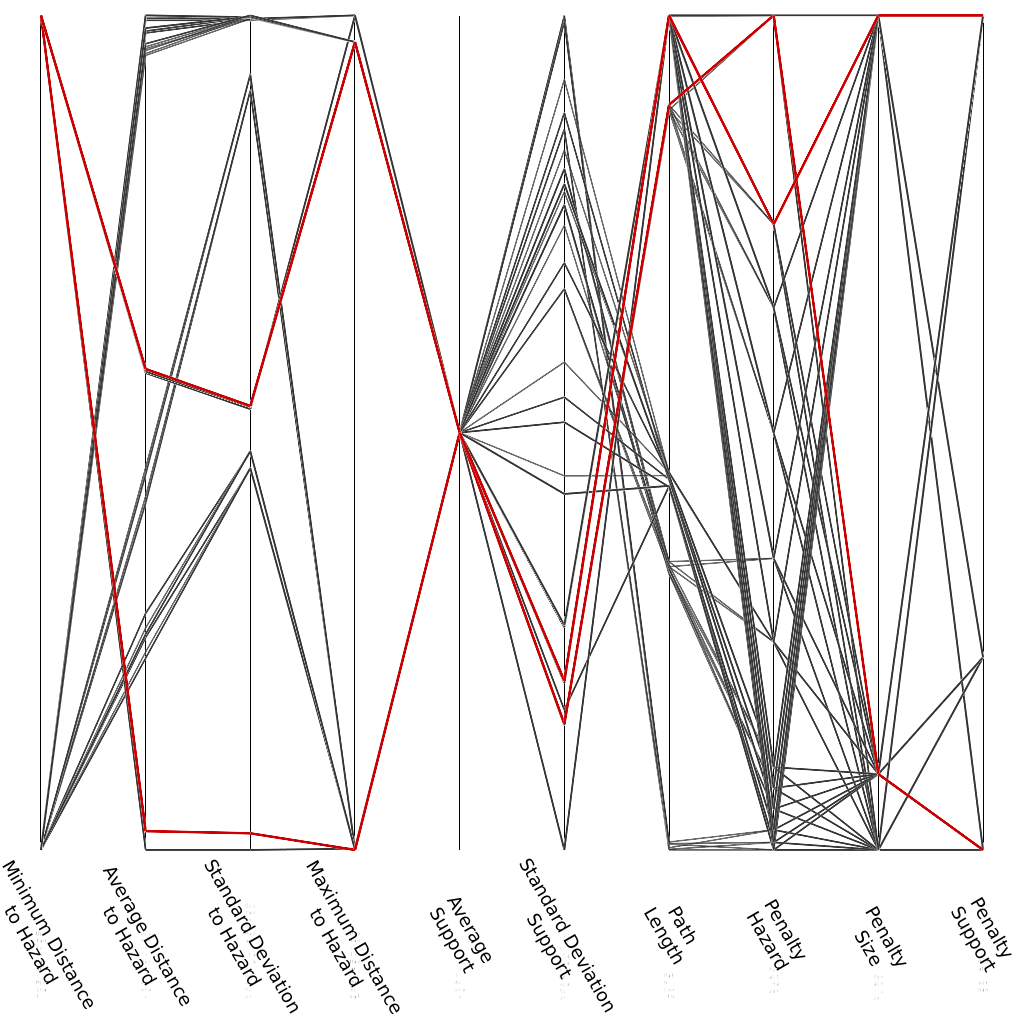
\includegraphics[width=\mysize]{figures/fig-analysis-pcp.png}
	    }
	    \label{fig:overview:analysis:pcp}
	}
	\subfigure[Scatter Plot Matrix]{
	    \framebox[\mysize][c]{
	        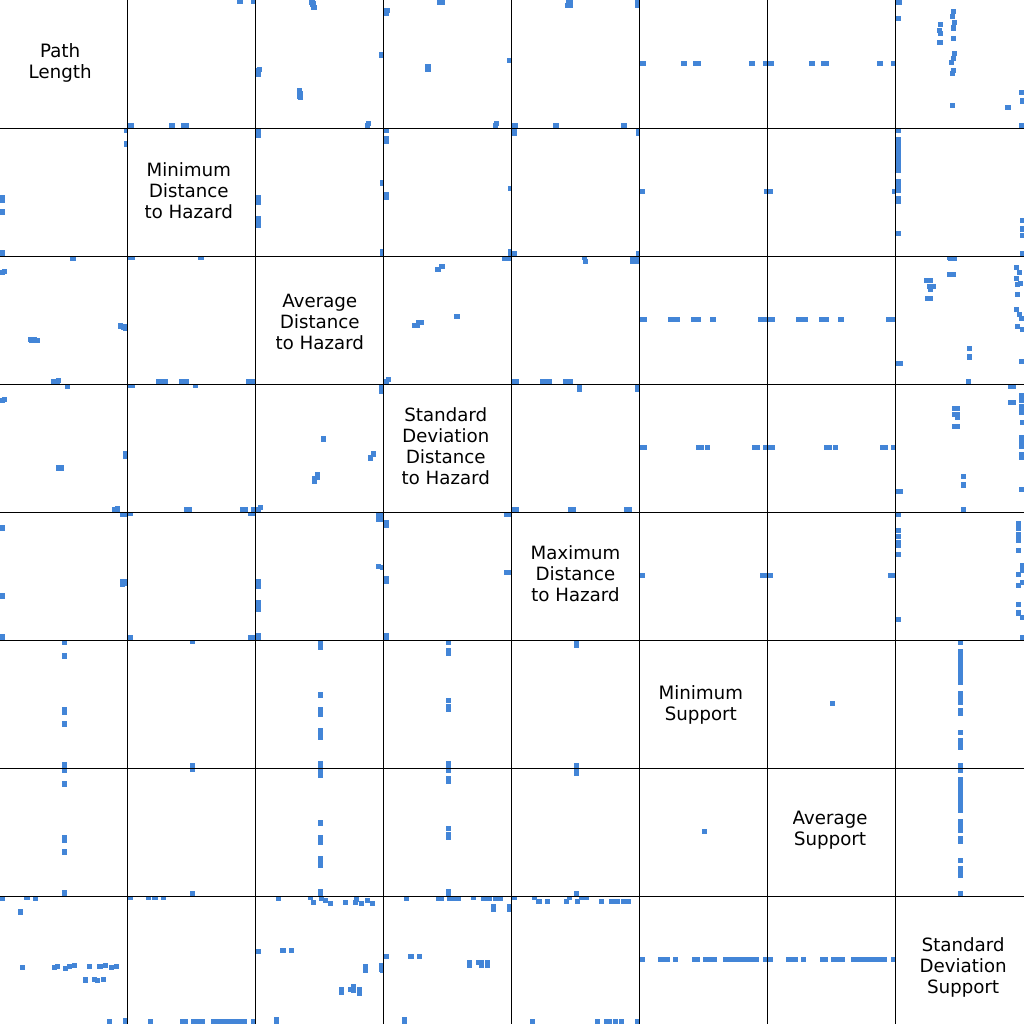
\includegraphics[width=\mysize]{figures/fig-analysis-scatter.png}
	    }
	    \label{fig:overview:analysis:scatter}
	}
	\subfigure[Profile Plot]{
	    \framebox[\mysize][c]{
	        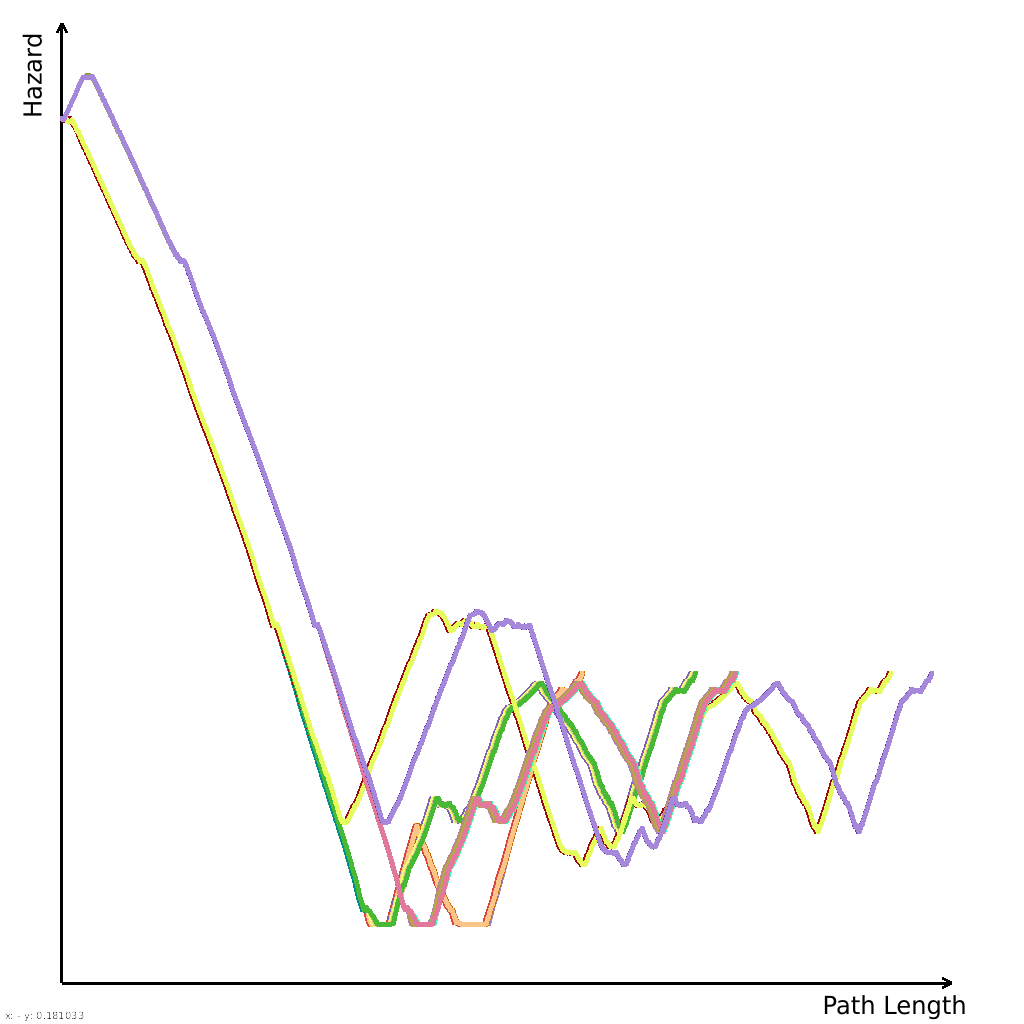
\includegraphics[width=\mysize]{figures/fig-analysis-profile.png}
	    }
	    \label{fig:overview:analysis:profile}
	}
    \caption{Screenshots of the analysis views in our system. (a) parallel coordinates plot with one of the paths selected. (b) scatter plot matrix depicting the correlations of all attributes. (c) distance to the closest hazard over path length.}
\end{figure*}

In order to enable informed trade-offs between all computed paths and selecting one suitable path, it is essential to provide detailed information about the various paths in a way that is easy to interpret. In this section we will explain the different views accessible by the \IC\ to gain a deeper understanding of the data. All views utilize the same brushing and linking features.

The \IC\ can use these methods to filter the large number of computed paths so that he can make an informed decision about an optimal trade-off. These trade-offs depend on the specific situation and experience of the \IC\ but include travel distance versus proximity to hazards or inclination of the walking surface versus available support among others. Because the exact details of the trade-offs depend on the \IC, we provide adaptive tools to filter and analyze the data according to information the \IC\ requests. This allows him to make full use of his knowledge in a strategic decision making scenario.

\subsubsection{Parallel Coordinates Plot} \label{sec:overview:analysis:pcp}
Parallel Coordinates Plots (PCP)~\cite{146402} are a visualization technique to inspect multidimensional data. It is very well suited to detect regularities and patterns in the data and deviations from these patterns and also enhances interactive exploration of data sources~\cite{Tory05aparallel}.

Figure~\ref{fig:overview:analysis:pcp} shows the PCP in our system with each computed path represented by one line. The axes are grouped into \emph{derived attributes}, like path length, minimal distance to hazard, average distance to hazard, or standard deviation of support, and \emph{path parameters} that were used to compute the path in question. While the first group is used to perform the necessary trade-off between paths, the second group is primarily used to filter the data. The \IC\ can select which attributes and parameters are visible in the PCP.  Through exploration of parameters, the \IC\ can move from mental simulation of alternatives, to simulation supported by the decision support system, thus amplifying RPD. The ability to explore trade-offs between alternative paths should facilitate a strategic COCOM decision mode, for the targeting ECOM level. In addition to filtering of paths, which is replicated in all other views, the \IC\ can select a path in this view and the selection is also linked in the system. Detecting previously unknown correlations and the ability to filter large parts of the data quickly helps to fulfil requirements {\bfseries R3} and {\bfseries R4}.

\subsubsection{Scatter Plot Matrix} \label{sec:overview:analysis:scatter}
The PCP is primarily used for those aspects that we foresee that the \IC\ wants to compare frequently. However, in line with the literature on resilience engineering~\cite{Lundberg2012} we also provide comparisons that cannot be foreseen in advance. Therefore we present attributes in a Scatter Plot Matrix (SPLOM), where each variable is given a row of scatter plots that show relations to all other variables. It allows the \IC\ to make comparisons opportunistically, zooming in on the required comparisons if needed. Each individual scatter plot shows the correlation between two attributes and can be used by the \IC\ to verify known relationships or discover new interactions~\cite{Li2008}. In addition, paths selected in this view are linked to the other views providing a consistent representation of the available paths. Figure~\ref{fig:overview:analysis:scatter} shows the SPLOM during usage.

\subsubsection{Profile Plot} \label{sec:overview:analysis:profile}
PCP and SPLOM are useful to inspect attributes that are valid for the path as a whole. In order to enable detailed analyses of values that change along the path, we include a profile plot. This is a variation of a line plot with different attributes over the path length enabling the \IC\ to spot outliers among the paths. This view makes it easy to compare the paths with regard to the chosen variable, as minima and maxima over all paths are easy to detect. Furthermore, it allows the \IC\ to spot irregularities along the path due to measurement errors, which would present themselves as single spikes. Having the possibility to detect these spikes, it is possible to fix the measurement errors and come to a more accurate path description. In Figure~\ref{fig:overview:analysis:profile} hazard distance profiles for a set of already filtered paths are shown. 

\subsection{Rendering} \label{sec:overview:rendering}
\noindent {\bfseries Point Cloud Rendering.} Rendering the unfiltered point cloud proved to be insufficient in early tests as missing depth cues and surface occlusion inhibited the necessary immersion. A voxelized representation is beneficial, as rendering each voxel using axis-aligned boxes solves the occlusion problem immediately (Figure~\ref{fig:teaser:1}). Holes appear in the rendering only in cases with very sparse data. To increase the spatial awareness, we apply an illumination technique to the rendering, where the lighting is based on the face normal of the voxel, rather than the normal of the voxel as computed in Section~\ref{sec:overview:precomputation}. We use the face normal as it is completely stable and constant for a given surface, thus making surfaces easier to detect. The \IC\ can add clip planes, for example to remove ceilings, to deal with unwanted occlusion in the scene.

\noindent {\bfseries Path Rendering.} In order for the user to understand the spatial relationship of the paths, it is useful and necessary to show the paths embedded in the rendering. Since the paths are computed based on the center points of the voxels, it is necessary to increase the $y$ value of each control point by at least half the voxel size in $y$ direction. In our experiments, we found that increasing it by about 2--3 times the voxel size produces a good visual result without looking too detached.

The \IC\ can select different coloring to inspect the stored information about the paths. Since the rendering view can become very cluttered, it is possible for the user to select a path in the rendering, which highlights that path in all other linked views and desaturates all other paths. Thus, it is possible to inspect the exact behavior of a few paths without distraction and also allows the user to reduce the number of considered paths very quickly.

Rather than relying on a mental simulation of the situation, the \IC\ can use a virtual walkthrough to inspect whether a plan will actually work. This walkthrough can either be interactively steered by the \IC\ or the camera can follow a chosen path automatically. Through looking at the information, the \IC\ can use his own experience to judge whether a path is likely to be passable.